
\documentclass[11pt]{report} % use larger type; default would be 10pt
%\documentclass[twocolumn]{book}
%\documentclass[twocolumn]{article}
%\documentclass[12pt]{book}
%\documentclass[11pt]{article}
%\documentclass[twocolumn, 12pt]{book}

%Pour écrire du français.
\usepackage[francais]{babel}
\usepackage[utf8]{inputenc}
\usepackage[T1]{fontenc}

%Police conseillée pour les pdf
\usepackage{lmodern}

%Choisir le format de sortie.
\usepackage{geometry} % to change the page dimensions
\geometry{a4paper} % or letterpaper (US) or a5paper or....
%\usepackage[top=2cm, bottom=2cm, left=2cm, right=2cm]{geometry}
% \geometry{margin=2in} % for example, change the margins to 2 inches all round
% \geometry{landscape} % set up the page for landscape
%   read geometry.pdf for detailed page layout information

\usepackage{setspace}

%Images incrustées
\usepackage{wrapfig}

%Tableaux
\usepackage{multirow}
\usepackage{slashbox}
\usepackage{colortbl}
\usepackage{color}


%euros
\usepackage{eurosym}

%Maths
\usepackage{amsmath}
\usepackage{amssymb}
\usepackage{mathrsfs}
\usepackage{amsthm}

%index
\usepackage{makeidx}

%url
\usepackage{url}

%Connaitre la dernière page
\usepackage{lastpage}

%lien hypertext
\usepackage{hyperref}
\hypersetup{
colorlinks=true, % Allow links color
urlcolor= blue, % Hyperlinks color
linkcolor= black, % Internal links color
}

\usepackage{graphicx} % support the \includegraphics command and options

% \usepackage[parfill]{parskip} % Activate to begin paragraphs with an empty line rather than an indent

%%% PACKAGES
\usepackage{booktabs} % for much better looking tables
\usepackage{array} % for better arrays (eg matrices) in maths
\usepackage{paralist} % very flexible & customisable lists (eg. enumerate/itemize, etc.)
\usepackage{verbatim} % adds environment for commenting out blocks of text & for better verbatim
\usepackage{subfig} % make it possible to include more than one captioned figure/table in a single float

%%%Personal packages
\usepackage{moreverb}
\usepackage{latexsym}
\usepackage{framed}

\usepackage{xcolor}
\usepackage{listings}
\usepackage{caption}
\DeclareCaptionFont{white}{\color{white}}
\DeclareCaptionFormat{listing}{%
  \parbox{\textwidth}{\colorbox{gray}{\parbox{\textwidth}{#1#2#3}}\vskip-4pt}}
\captionsetup[lstlisting]{format=listing,labelfont=white,textfont=white}
\definecolor{mygreen}{rgb}{0,0.6,0}
\definecolor{mygray}{rgb}{0.5,0.5,0.5}
\definecolor{mymauve}{rgb}{0.58,0,0.82}
\lstset{frame=lrb,xleftmargin=\fboxsep,xrightmargin=-\fboxsep}

\lstset{ %
language=Java, % choose the language of the code
basicstyle=\footnotesize, % the size of the fonts that are used for the code
backgroundcolor=\color{white}, % choose the background color. You must add \usepackage{color}
showspaces=false, % show spaces adding particular underscores
showstringspaces=false, % underline spaces within strings
showtabs=false, % show tabs within strings adding particular underscores
frame=single, % adds a frame around the code
tabsize=4, % sets default tabsize to 2 spaces
captionpos=t, % sets the caption-position to bottom
breaklines=true, % sets automatic line breaking
breakatwhitespace=false, % sets if automatic breaks should only happen at whitespace
keywordstyle=\color{blue},
stringstyle=\color{mymauve},
rulecolor=\color{black},
extendedchars=true, belowcaptionskip=3ex,
numbers=left,
escapeinside={\%*}{*)} % if you want to add a comment within your code
}


% These packages are all incorporated in the memoir class to one degree or another...

%%% HEADERS & FOOTERS
\usepackage{fancyhdr} % This should be set AFTER setting up the page geometry

\pagestyle{fancy} % options: empty , plain , fancy
\renewcommand{\headrulewidth}{0pt} % customise the layout...
\lhead{}\chead{}\rhead{}
\lfoot{}\cfoot{\thepage}\rfoot{}

%%% SECTION TITLE APPEARANCE
\usepackage{sectsty}
\allsectionsfont{\sffamily\mdseries\upshape} % (See the fntguide.pdf for font help)
% (This matches ConTeXt defaults)

%%% ToC (table of contents) APPEARANCE
\usepackage[nottoc,notlof,notlot]{tocbibind} % Put the bibliography in the ToC
\usepackage[titles,subfigure]{tocloft} % Alter the style of the Table of Contents
\renewcommand{\cftsecfont}{\rmfamily\mdseries\upshape}
\renewcommand{\cftsecpagefont}{\rmfamily\mdseries\upshape} % No bold!


%%% END Article customizations















%%% The "real" document content comes below...

\title{Rapport de projet}
\author{\textsc{Wollenburger} Antoine, \textsc{Chénais} Sébastien}
\date{} %Hide the date

\begin{document}
%Pied de page et entête (Un peu trop non ?) www.siteduzero.com/informatique/tutoriels/redigez-des-documents-de-qualite-avec-latex/les-styles-4
%Annule tous les trucs de base
\fancyhead[LE,CE,RE,LO,CO,RO]{}
\fancyfoot[LE,CE,RE,LO,CO,RO]{}

%Personnalisation
\fancyhead[LO, LE]{Rapport de programmation}
\fancyhead[RO,RE]{Page \thepage \ sur \pageref{LastPage}}
%\fancyfoot[LO,LE]{Université de \scshape{Nantes}}
%\fancyfoot[RO,RE]{Page \thepage \ sur \pageref{LastPage}}
%Lignes
\renewcommand{\headrulewidth}{0.4pt}
%\renewcommand{\footrulewidth}{0.4pt}

\maketitle

%Table des matières
\renewcommand{\contentsname}{Sommaire} % Dans le corps du document,avant la commande \tableofcontents.
\tableofcontents

\addcontentsline{toc}{chapter}{Introduction}
\chapter*{Introduction}
Il nous a été demandé d'écrire un compilateur, en OCAML, d'un langage de notre cru vers du svg (format pour décrire des images vectorielles). Pour mener à bien cette tâche, nous nous reposerons sur les notions que nous avons vues en cours.

Pour rappel, une image vectorielle est une image dont les éléments sont définis individuellement sous forme d'objet géométrique. Elle se différencie d'une image matricielle qui utilise des pixels. Son principal avantage est qu'elle peut être agrandie à l'infini sans perte de qualité contrairement à une image matricielle. Son inconvénient est que pour atteindre une qualité photo-réaliste, il faut beaucoup de ressource, l'image étant calculée à chaque affichage.

\begin{figure}[h]
    \centering
    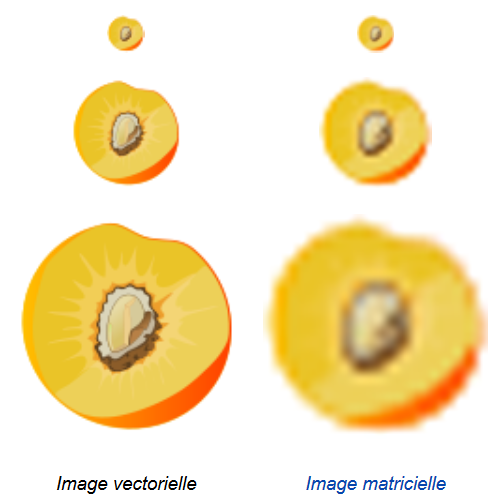
\includegraphics[scale=0.7]{img/SVG_vs_BMP.png}
    \caption{\label{CG} SVG contre Matriciel. \href{http://fr.wikipedia.org}{fr.wikipedia.org}}
\end{figure}

\chapter{Analyse lexicale et syntaxique de SVGgenerator}

Cette section a pour but la définition du langage SVGgenerator et de sa grammaire associée. 
\section{Définition d'une grammaire}
La première étape de ce projet a été la création d'un langage et sa grammaire associée. Même si le projet global se fera de manière incrémentale, il faut penser au fonctionnement global dès le début. 

\subsection{Définition d'une image vectorielle}

Le fichier SVG est déclaré par l'instruction "drawing" suivi du nom du dessin et la taille du canevas sous la forme "[largeur , hauteur]". Les instructions sont incluses entre les crochets.

\begin{lstlisting}[caption=Définition d'une image vectorielle, language=C]
drawing monDessin [256 , 256]
{
    -instructions-
}
\end{lstlisting}

\subsection{Les instructions}
Une instruction peut être de différents types:
\begin{description}

  \item[Une déclaration de variable]: on créé une variable en indiquant son type, son nom et enfin les valeurs qui servent à la construire.

\begin{minipage}{\linewidth}
\begin{lstlisting}[caption=Déclaration de variable, language=C]
Type ma_Variable( -param- );
\end{lstlisting}
\end{minipage}

  \item[Le dessin d'une variable]: pour les variables dont le type est adéquat, il s'agit de l'instruction qui déclenche l'affichage de ladite variable. La forme est "draw nomDeLaVariable".

\begin{minipage}{\linewidth}
\begin{lstlisting}[caption=Dessin d'une variable, language=C]
draw ma_Variable;
\end{lstlisting}
\end{minipage}




 \item[Une boucle]: il s'agit d'une boucle itérative. L'instruction est de la forme "For(var=start,end)\{\}". Le bloc entre crochets est répété tant que le compteur n'a pas atteint la valeur "end" (il est à noter que ce compteur, bien que pouvant être utilisé dans le corps de la boucle, doit être déclaré avant la boucle, et que toute modification l'affectant n'influera pas sur le nombre d'étapes de la boucle).

\begin{minipage}{\linewidth}
\begin{lstlisting}[caption=Boucle, language=C]
Float i(0);
For(i=start,end) {
	- instructions-
};
\end{lstlisting}
\end{minipage}
 % \item[Une boucle]: il s'agit d'une boucle sur condition. L'instruction est de la forme "while(-conditions-)\{\}". Le bloc entre crochets est répété jusqu'à ce que la condition soit invalidée.

%\begin{minipage}{\linewidth}
%\begin{lstlisting}[caption=Boucle, language=C]
%while( -condition- ){
%	-instructions-
%}
%\end{lstlisting}
%\end{minipage}

  \item[Les fonctions et procédures]: il s'agit d'un appel a une fonction ou une procédure. L'instruction est de la forme "nomDeLaFonction (-paramètres-)". Pour les fonctions, il est possible de récupérer une valeur de retour.

\begin{minipage}{\linewidth}
\begin{lstlisting}[caption=Fonctions et procédures, language=C]
ma_fonction (-param-);
\end{lstlisting}
\end{minipage}

\end{description}

Quelques instructions n'ont pas encore été implémentées. Voici comment nous aurions procédé le cas échéant : 

\begin{description}
  \item[Une conditionnelle]: il s'agit d'un test sur une ou plusieurs conditions qui influe sur la suite de l'exécution. Cette instruction est de la forme "if(-conditions-)\{\}else\{\}". Si la condition est vérifiée, alors le bloc correspondant au if est exécuté, celui correspondant au else sinon.

\begin{minipage}{\linewidth}
\begin{lstlisting}[caption=Conditionnelle, language=C]
if( -condition- ){
	- instructions-
}
else{
	-instructions-
}
\end{lstlisting}

Son implémentation nécessite deux choses : 
\begin{itemize}
\item L'ajout des booléens, et de leurs opérateurs logiques. Cette étape est des plus bénigne, tant ce modèle est proche de celui des expressions arithmétiques.
\item L'ajout de la conditionnelle : il eu fallu ajouter les tokens, les règles de parsage, et enfin une action utilisant le if de caml et nos booléens (fonction execute\_action\_before)
\end{itemize}
\end{minipage}

\item[Ajout de propriétés aux objets]: %TODO couleur,... pas géré, comment faire

\end{description}
Seuls le manque flagrant de temps et la proximité des examens nous ont empêchés de les implémenter.

\subsection{Les types}
Plusieurs types ont été définis à l'origine:
\begin{description}
\item[Float]: Il s'agit d'un nombre. Son interprétation interne sera le flottant.
\item[Point]: Un Point est défini par deux Number correspondant à l'abscisse et l'ordonnée. Sa représentation en SVG est inexistante.
\item[Line]: Une Line est définie par deux points correspondant au début et à la fin de la Line. Sa représentation en SVG est une ligne.
\item[Rectangle]: Un Rectangle est défini par un Point et deux Number, correspondant respectivement à une des extrémité de la forme, à la longueur et la largeur. Sa représentation en SVG est le rectangle.
\item[Circle]: Un Circle est défini par un point et un Number, correspondant respectivement au centre et au rayon de la forme. Sa représentation en SVG est le cercle.
\end{description}

\subsection{Les commentaires}
Le langage autorise les commentaires sous deux formes. Premièrement, le commentaire sur une ligne qui commence par "//". Ce commentaire peut être placé en début ou en fin de ligne. Enfin, le commentaire sur plusieurs lignes encadré par "/*" et "*/". Toutes les instructions commentées ne sont pas interprétées.
\begin{lstlisting}[firstnumber=1][caption=Commentaires, language=C]
//ceci est un commentaire sur une ligne
/* ceci est
un commentaire en
bloc */
-instruction- //commentaire
\end{lstlisting}

\subsection{La grammaire}
Voici la grammaire associée à SVGgenerator.
\begin{lstlisting}[caption=Grammaire associée a SVGgenerator, language=C]
Grammaire SVGgenerator{S,Vt,Vn,R}

Vt = { 'drawing'; '['; ']'; 'x'; '{'; '}'; 'Point'; '('; ','; ')'; ';'; 'Line'; 'draw'; 'var'; 'number'; 'eof'; '+'; '-'; '/'; '*'; '.';'='; 'Rect'}
Vn = {S; Bloc{; Instructions; Instr; Declaration; Draw; Function; Param; Exp_ar; Var; T; F; Affectation; Subvar}

R{
S				-> Function.Drawing.'eof'
S				-> Drawing.'eof'
Function		-> 'function'.'var'.'('.Param.')'.Bloc{
Function		-> 'function'.'var'.'('.Param.')'.Bloc{.Function
Param			-> Param.','.Param
Param			-> 'Point'.'var'
Param			-> 'Line'.'var'
Drawing			-> 'drawing'.'var'.'['.'number' ',' 'number'.']'.Bloc{
Bloc{			-> '{'.Instructions.'}'
Instructions	-> Instr.Instructions
Instructions	-> Instr
Instr			-> Declaration
Instr			-> Draw
Instr			-> Fun
Declaration		-> 'Point'.'var'.'('.Exp_ar.','.Exp_ar.')'.';'
Declaration		-> 'Line'.'var'.'('.'var'.','.'var'.')'.';'
Declaration		-> 'Float'.'var'.'('.'Exp_ar'.')'.';'
Declaration		-> 'Rect'.'var'.'('.'var'.','.'Exp_ar'.','.Exp_ar.')'.';'
Draw			-> 'draw'.'var'.';'
Affectation		-> Subvar.'='.Exp_ar.';'
Affectation		-> Subvar.'='.Subvar.';'
For				-> 'for'.'('.'var'.'='.Exp_ar.','.Exp_ar.')'.Bloc{
Fun 			-> 'var'.'('.Var.')'.';'
Fun 			-> 'var'.'('.Exp_ar.')'.';'
Var				-> 'var'.','.Var
Var				-> 'var'
Exp_ar 			-> T.'+'.Exp_ar
Exp_ar 			-> T.'-'.Exp_ar
Exp_ar			-> T
T				-> F.'*'.T
T				-> F.'/'.T
T				-> F
F				-> 'number'
F				-> '('.Exp_ar.')'
Subvar			-> Subvar.'.'.'var'
Subvar			-> 'var'
}
\end{lstlisting}

\section{L'analyse lexicale}
	L'analyse lexicale est effectuée au niveau du fichier grapheur\_lexer.mll. Nous identifions le vocabulaire terminal Vt tel que déclaré dans la grammaire. C'est a cet endroit que nous gérons les commentaires en ignorant tout entrée entre '/*' et '*/' ainsi que toute entrée entre '/' et une fin de ligne.

De même, nous ignorons tout caractère de type espace, tabulation ou retour charriot.

Un nom de variable est composé d'une lettre puis éventuellement d'une liste de lettre et nombre, quelle que soit la casse.

Un nombre correspond à un flottant de la forme X ou X.X où X est un entier.

Les tokens étant crées, il faut maintenant analyser leur syntaxe.

\section{L'analyse syntaxique}
L'analyse syntaxique à pour objectif la création d'une structure utilisable pour la génération du fichier SVG. Cette structure est un arbre binaire comme défini à la suite. Chaque n{\oe}ud correspond à une opération qui peut être un token, un nom de variable ou un nombre.

\begin{lstlisting}[caption=Type arbre, language=caml]
type operation =
    Drawing
  | Root
  | Function
  | Functions
  | DrawingSize
  | BlocEmbrace
  | Declaration
  | BlocBrace
  | BlocPar
  | Parameters
  | Parameter
  | ParametersUse
  | ParameterUse
  | FunctionUse
  | Point
  | Float
  | Line
  | Rect
  | Instruction
  | Comma
  | Draw
  | Moins
  | Plus
  | Mult
  | Div
  | For
  | Dot
  | Affectation
  | Arithm_expr
  | Var of (string)
  | Number of (float);;
  
type t_arbreB = Empty | Node of node
        and node = { value: operation; left: t_arbreB; right: t_arbreB };;
\end{lstlisting}

Voici une représentation visuelle de l'arbre,  n{\oe}ud par  n{\oe}ud. Un n{\oe}ud de couleur verte signifie qu'il s'agit de la tête de son arbre. Un n{\oe}ud de couleur rouge représente un n{\oe}ud non final, à relier à un n{\oe}ud vert.

\begin{figure}[h]
    \centering
    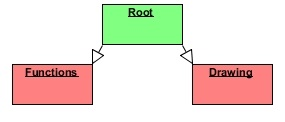
\includegraphics[scale=1]{img/root.jpg}
    \caption{\label{CG} Root - tête de l'arbre général.}
\end{figure}
\begin{figure}[h]
    \centering
    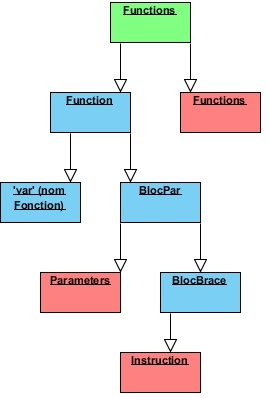
\includegraphics[scale=1]{img/functions.jpg}
    \caption{\label{CG} Functions - tête pour chaque.}
\end{figure}
\begin{figure}[h]
    \centering
    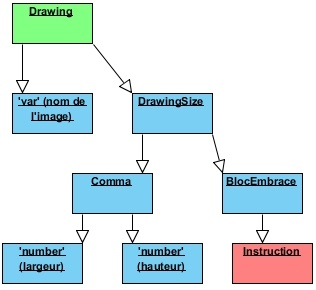
\includegraphics[scale=1]{img/drawing.jpg}
    \caption{\label{CG} Drawing - tête pour le dessin.}
\end{figure}
\begin{figure}[h]
    \centering
    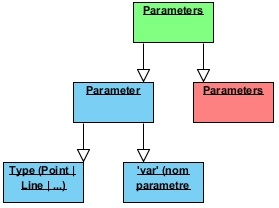
\includegraphics[scale=1]{img/parameters.jpg}
    \caption{\label{CG} Parameters - tête pour une suite de paramètres.}
\end{figure}
\begin{figure}[h]
    \centering
    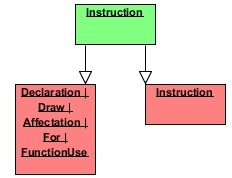
\includegraphics[scale=1]{img/instruction.jpg}
    \caption{\label{CG} Instruction - tête pour une suite d'instruction.}
\end{figure}
\begin{figure}[h]
    \centering
    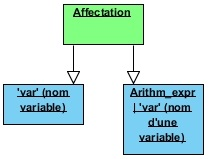
\includegraphics[scale=1]{img/affectation.jpg}
    \caption{\label{CG} Affectation - tête pour une affectation de variable.}
\end{figure}
\begin{figure}[h]
    \centering
    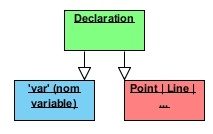
\includegraphics[scale=1]{img/declaration.jpg}
    \caption{\label{CG} Déclaration - tête pour une déclaration de variable.}
\end{figure}
\begin{figure}[h]
    \centering
    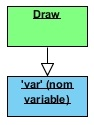
\includegraphics[scale=1]{img/draw.jpg}
    \caption{\label{CG} Draw - tête pour le dessin d'une variable.}
\end{figure}
\begin{figure}[h]
    \centering
    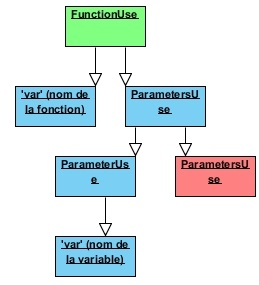
\includegraphics[scale=1]{img/fonctionuse.jpg}
    \caption{\label{CG} FunctionUse - tête pour l'appel à une fonction.}
\end{figure}
\begin{figure}[h]
    \centering
    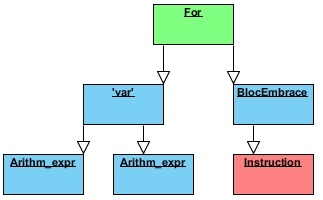
\includegraphics[scale=1]{img/for.jpg}
    \caption{\label{CG} For - tête pour une boucle for.}
\end{figure}




\chapter{Génération du code SVG}

\section{Les variables}

\subsection{affectation}

Pour être utilisée dans la suite du programme, une variable doit être déclarée. Dans notre cas, la déclaration s'accompagne aussi d'une affectation. Il est par conséquent impossible de crée une variable nulle. Les variables sont stockées au fur et à mesure de leur apparition dans une hash table, d'une taille arbitraire de 1000. La clé est donc le nom ce qui peut poser problème lors de l'utilisation des fonctions. Pour y remédier, lorsqu'on sort d'un domaine de visibilité (représentés par un bloc de  \{\}), les variables déclarées dans ce bloc sont supprimées. Ainsi, les variables déclarée dans le bloc général (drawing) sont globales par rapport aux fonctions. Si une fonction possède une variable du même nom, la variable de la fonction sera utilisée. La valeur associée à la clé est le type de la variable.
Si une même variable est déclarée deux fois, le compilateur génère une erreur. 

\subsection{réutilisation}

Lors de l'appel à une variable, sa valeur est recherchée dans la table. Si la valeur est présente et le type adéquat à la situation, l'exécution se poursuit. Sinon, le compilateur génère une erreur. Pour les types primitifs, ici Float, la variable est remplacé par sa valeur.

\subsection{les objets}

En dehors du Float, chaque type de variable correspond à un objet (Rect, Point,...). Ces objets ont des attributs de type primitif ou objet. Il est possible d'atteindre ces attributs à l'aide du '.' (point). Voici ces attributs:
\begin{description}
\item[Point]: x et y de type Float.
\item[Line]: p1 et p2 de type Point.
\item[Rectangle]: o de type Point et w,h de type Float.
\end{description}

Ex :
monPoint.x;

L'affectation et la réutilisation des attributs est possible.

\section{Les opérations arithmétiques}

Cette section va être succincte, les opérations arithmétiques étant un cas d'étude fréquent. 

Elles sont faisable partout excepté lors de l'appel à une fonction. En effet, la fonction effectue une vérification de type avant de s'exécuter, et le type d'une opération arithmétique n'est pas Float tant qu'on ne la pas résolue. C'est un problème à régler.

\section{les fonctions}



\chapter{Le langage, spécificités, contraintes} %linkage, appel aux fonctions (pré calcul,...)

\appendix

\chapter{Journal des évolutions}
\section{Lexer}
\section{Parser : vers un arbre pour représenter le fichier}
\section{Interlude : table S-R et inutilité}

\section{De l'exploitation de l'arbre}
\subsection{Lecture du drawing}%Powa : un fichier svg vide
\subsection{Déclaration de procédures}
\subsection{La déclaration de variables} %Caml objects, ....
\subsection{De l'utilisation des procédures}%recopie,....
\subsection{Principe d'actions} %exécution du code
\subsection{Les 0.}

\section{Le boulversement FOR}
\subsection{L'idée du for}
\subsection{Ajout des floats}
\subsection{L'arrivée de la notion de visibilité}
\subsection{Réunification du préparsage et de l'exécution}
\subsection{La réalité du FOR}

\section{La visiblité devient générale}

\section{Interlude : liens entre objets}
\section{Opérations sur les objets}
\subsection{Récupération de la valeur}
\subsection{Affectation d'une valeur}

\section{L'ajout d'objets, simplicité}
\subsection{Déclaration}
\subsection{Opérations}
\subsection{Dessin}


\end{document}